% -----------------------------------------------
% Template for ISMIR Papers
% 2021 version, based on previous ISMIR templates

% Requirements :
% * 6+n page length maximum
% * 10MB maximum file size
% * Copyright note must appear in the bottom left corner of first page
% * Clearer statement about citing own work in anonymized submission
% (see conference website for additional details)
% -----------------------------------------------

\documentclass{article}
\usepackage[T1]{fontenc} % add special characters (e.g., umlaute)
\usepackage[utf8]{inputenc} % set utf-8 as default input encoding
\usepackage{ismir,amsmath,cite,url}
\usepackage{graphicx}
\usepackage{color}


\usepackage{lineno}
\linenumbers

% Title. Please use IEEE-compliant title case when specifying the title here,
% as it has implications for the copyright notice
% -----
\title{Revisiting ``Shallow'' Music Representation Learning with HDPGMM}

% Note: Please do NOT use \thanks or a \footnote in any of the author markup

% Single address
% To use with only one author or several with the same address
% ---------------
%\oneauthor
% {Names should be omitted for double-blind reviewing}
% {Affiliations should be omitted for double-blind reviewing}

% Two addresses
% --------------
%\twoauthors
%  {First author} {School \\ Department}
%  {Second author} {Company \\ Address}

% Three addresses
% --------------\input{ISMIR2021_paper.tex}

\threeauthors
  {First Author} {Affiliation1 \\ {\tt author1@ismir.edu}}
  {Second Author} {\bf Retain these fake authors in\\\bf submission to preserve the formatting}
  {Third Author} {Affiliation3 \\ {\tt author3@ismir.edu}}

% Four or more addresses
% OR alternative format for large number of co-authors
% ------------
%\multauthor
%{First author$^1$ \hspace{1cm} Second author$^1$ \hspace{1cm} Third author$^2$} { \bfseries{Fourth author$^3$ \hspace{1cm} Fifth author$^2$ \hspace{1cm} Sixth author$^1$}\\
%  $^1$ Department of Computer Science, University , Country\\
%$^2$ International Laboratories, City, Country\\
%$^3$  Company, Address\\
%{\tt\small CorrespondenceAuthor@ismir.edu, PossibleOtherAuthor@ismir.edu}
%}

% For the author list in the Creative Common license, please enter author names. 
% Please abbreviate the first names of authors and add 'and' between the second to last and last authors.
\def\authorname{F. Author, S. Author, and T. Author}

% Optional: To use hyperref, uncomment the following.
%\usepackage[bookmarks=false,pdfauthor={\authorname},pdfsubject={\papersubject},hidelinks]{hyperref}
% Mind the bookmarks=false option; bookmarks are incompatible with ismir.sty.

\sloppy % please retain sloppy command for improved formatting

\begin{document}

%
\maketitle
%
\begin{abstract}
The abstract should be placed at the top left column and should contain about 150-200 words.
\end{abstract}
%
\section{Introduction}\label{sec:introduction}

blah blah
%

\section{Related works}\label{sec:rel_works}

blah blah
%
\section{HDPGMM}\label{sec:hdpgmm}

In this subsection, we introduce the main model we employ for this study; the Hiararchical Dirichlet Process Gaussian Mixture Model (HDPGMM)~\cite{DBLP:conf/ismir/HoffmanBC08, doi:10.1198/016214506000000302}. To introduce the model properly it would be useful to start discussing the Dirichlet Process Mixture Model (DPMM), the model on which HDPGMM is extended.

\subsection{Dirichlet Process Mixture Models}\label{sec:hdpgmm:dpmm}

Mixture models such as GMMs assume a finite number of components from which each of observed feature vectors are drawn. It is well known that finding the optimal number $K$ of the mixuture components is a difficult problem. There are a few approaches that can be useful to estimate $K$ such as using the cross-validation. Dirichlet Process Mixture Model (DPMM) circumbents this problem by parametrizing the number of mixtures as part of the model. DP plays a central role for such models.

DP is a stochastic process which draws random probability distributions. Due to this property, it is often described as a distribution over distributions~\cite{DBLP:reference/ml/Teh17}. It can be also seen as the infinite dimensional generalization of the Dirichlet distributions~\cite{DBLP:reference/ml/Teh17}.
This aspect is the core building block of the Bayesian non-parametric models such as infinite mixture models. Setting DP as a prior distribution for the responsibility $\pi$ (also often referred as mixture probability) of mixture components allows the mixture model to infer both the relative weight among components and the appropriate number of maximum components for given observations.

Among a several ways to represent DP, we introduce the stick-breaking construction~\cite{sethuraman94}.
\footnote{Literature commonly chooses the Chinese Restaurant Process (CRP) for a illustrative metaphor for DP as it is intuitive and well explains various properties of DP~\cite{DBLP:reference/ml/Teh17}. We mainly discuss DP with the stick-breaking construction due to its further usage in the model inference within the work. For readers interested in other metaphorical descriptions of DP, we kindly refer them to~\cite{DBLP:reference/ml/Teh17, DBLP:conf/ismir/HoffmanBC08}}
Stick-breaking constructs DP in a simple and general manner. Formally, it is as follows:

\begin{equation}\label{eq:stick_breaking}
\begin{aligned}[c]
    \beta^{\prime}_{k} &\sim \text{Beta}(1, \gamma) \\
    \beta_{k} &= \beta^{\prime}_{k} \prod_{l=1}^{k-1} (1 - \beta_{l}^{\prime})
\end{aligned}
\qquad
\begin{aligned}[c]
    \phi_{k} &\sim H \\
    G_{0} &= \sum^{\infty}_{k=1} \beta_{k}\delta_{\phi_{k}}
\end{aligned}
\end{equation}
where two euqations in the left column represent the draw of infinite dimensional weight $\beta_{k}$ which sums to one. Notably, the distribution for $\beta$ is also referred as $\beta \sim \text{GEM}(\gamma)$~\cite{DBLP:journals/cpc/Pitman02}. In the right column, $H$ denotes the base distribution from which variable $\phi_{k}$ lying in some space $\Phi$ is drawn. The right bottom equation defines the draw of the probability measure $G_{0}$, where $\delta_{\phi_{k}}$ means the point mass centered at the component $\phi_{k}$. Altogether, Eq. \ref{eq:stick_breaking} constructs the DP $G_{0} \sim \text{DP}(\gamma, H)$. Figure \ref{fig:stick_breaking} depicts the process in graphical way.

\begin{figure}[ht]
    \centering
    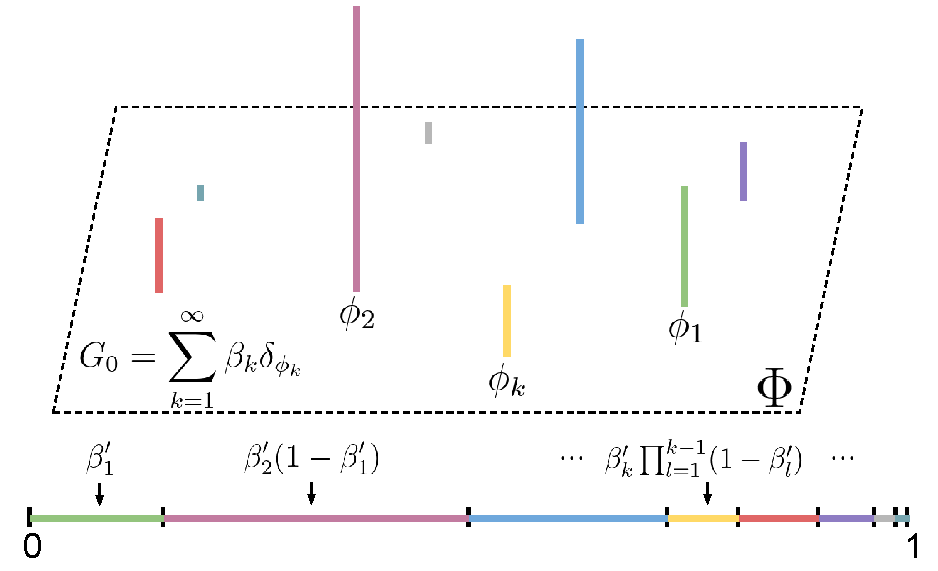
\includegraphics[width=0.9\linewidth]{figs/stick-breaking.pdf}
    \caption{Illustration of stick-breaking construction in Eq. \ref{eq:stick_breaking}}
    \label{fig:stick_breaking}
\end{figure}

In mixture model context, we want to infer mixture components $\{\phi_{1}, \phi_{2}, \cdots, \phi_{k}, \cdots\}$ that fits to the data observations $\{x_{1}, x_{2}, \cdots, x_{n}\}$, which are assumed to be drawn from distributions $F(\phi)$ parameterized with variable $\phi$ (i.e., mean and covariance $\phi = \{\mu, \Sigma\}$ in case of the multivariate Gaussian $F$). we can now use DP to draw $\phi$ as $i$th mixture components corresponds to the $i$th observation $x_{i}$ by introducing the cluster assignment variable $y_{i} \sim \text{Mult}(\beta)$:


\begin{equation}\label{eq:dpmm}
\begin{aligned}[c]
    \beta|\gamma &\sim \text{GEM}(\gamma) \\
    y_{i}|\beta &\sim \text{Mult}(\beta)
\end{aligned}
\qquad
\begin{aligned}[c]
    \phi_{k}|H &\sim H \\
    x_{i}|y_{i},\{\phi_{k}\} &\sim F(\phi_{y_{i}}) 
\end{aligned}
\end{equation}
where $\phi_{y_{i}}$ denotes the component parameter $\phi$ indexed by assignment variable $y_{i}$ corresponding to the $i$th observation $x_{i}$.


\subsection{Hierarchical DPMM}\label{sec:hdpgmm:hdpmm}

In many data structure, groupings of atomic data points arise naturally (i.e., audio frames within a song, songs from an artist, words of a lyrics). Hierarchical DP (HDP) is an extention of DP modelling ``groupings'' by imposing group-level DPs derived from the ``global-level'' or ``corpus-level'' DP as the global pool of components~\cite{doi:10.1198/016214506000000302}. Following Sethuraman's stick-breaking construction~\cite{DBLP:journals/jmlr/WangPB11}, $j$th group-level DP can be expressed as follows:


\begin{equation}\label{eq:hdp_doc_level}
\begin{aligned}[c]
    \pi^{\prime}_{jt} &\sim \text{Beta}(1, \alpha_{0}) \\
    \pi_{jt} &= \pi^{\prime}_{jt} \prod^{t - 1}_{l = 1} (1 - \pi^{\prime}_{jl})
\end{aligned}
\qquad
\begin{aligned}[c]
    \psi_{jt} &\sim G_{0} \\
    G_{j} &= \sum^{\infty}_{t = 1} \pi_{jt}\delta_{\psi_{jt}}
\end{aligned}
\end{equation}
As seen above, HDP indeed appears as the recursion of multiple levels of DPs\footnote{It implies naturally that multiple levels are possible (i.e., corpus - author - document), if it suits to the data structure.}. Notably, the base distribution $G_{0}$ of each group-level DP is from the corpus-level DP. This relationship allows to map group-level atoms $\psi_{jt}$ to the corpus-level atoms $\phi_{k}$. Wang et al. introduce a series of indicator variables $c_{jt}$ which maps $\psi_{jt}$ and $\phi_{k}$ as follows\cite{DBLP:journals/jmlr/WangPB11}:


\begin{equation}\label{eq:psi2phi}
\begin{aligned}
    c_{jt} &\sim \text{Mult}(\beta) \\
    \psi_{jt} &= \phi_{c_{jt}}
\end{aligned}
\end{equation}
where $\beta$ is drawn from the corpus-level DP in Eq. \ref{eq:stick_breaking}. It simplifies the model as we do not need to explicitly represent $\psi_{jt}$~\cite{DBLP:journals/jmlr/WangPB11}.
Finally, we can represent HDPMM by introducing another indicator variable $z_{jn} \sim \text{Mult}(\pi_{j})$ for $n$th observation $x_{jn}$ within the $j$th group, similarly to Eq. \ref{eq:dpmm}:


\begin{equation}\label{eq:hdpmm}
\begin{aligned}[c]
    \pi_{j}|\alpha_{0} &\sim \text{GEM}(\alpha_{0}) \\
    z_{jn}|\pi_{j} &\sim \text{Mult}(\pi_{j})
\end{aligned}
\qquad
\begin{aligned}[c]
    \theta_{jn} = \psi_{jz_{jn}} &= \phi_{c_{jz_{jn}}}  \\
    x_{jn}|z_{jn}, c_{jt}, \{\phi_{k}\} &\sim F(\theta_{jn}) 
\end{aligned}
\end{equation}
where we use the indicator $z_{jn}$ to select $\psi_{jt}$, which eventually is mapped as $\phi_{c_{jz_{jn}}}$ that represents the parameter $\theta_{jn}$ to draw the observation $x_{jn}$. HDPGMM is then defined by simply setting $F$ as the (multivariate) Gaussian distribution and $H$ as one of distribution from which we can sample the mean and covariance (i.e., Gaussian-inverse Wishart distribution).


\begin{figure}[ht]
    \centering
    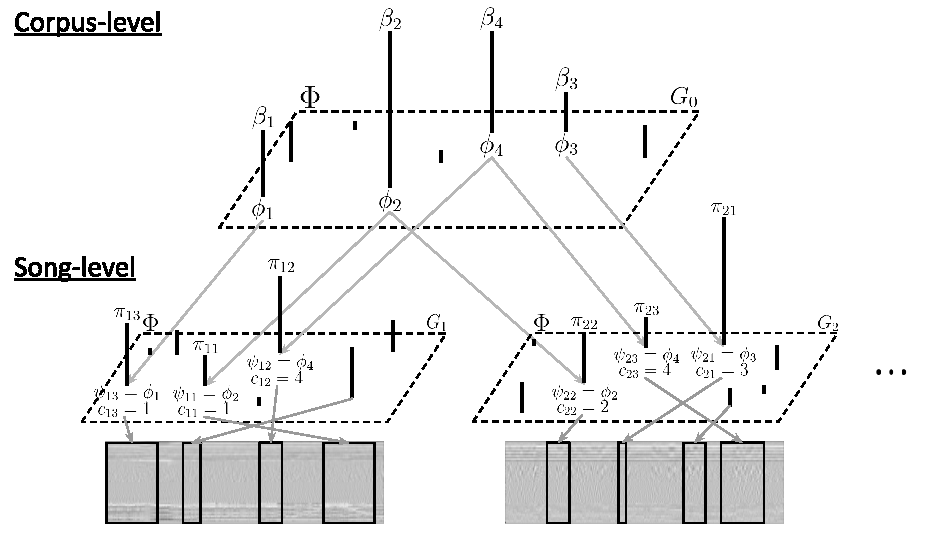
\includegraphics[width=\linewidth]{figs/HDP-stick-breaking.pdf}
    \caption{Illustration of 2-level HDPMM within corpus-song context. The top illustration depicts the corpus-level DP similar to Figure \ref{fig:stick_breaking}. The second row illustrations describe the draw of second level (song-level) DPs per song from the corpus-level DP. DPMM assumes that song features are drawn from each song-level DPs as depicted in the third rows of the image.}
    \label{fig:hdpmm}
\end{figure}


\subsection{Inference Algorithm}\label{sec:hdpgmm:inference}

In this section we discuss the inference (training) algorithm. We employ the online Variational Inference (VI)~\cite{DBLP:journals/jmlr/WangPB11}. VI is one of the common choices to infer a fully Bayesian models and usually significantly faster than other methods such as Markov Chain Monte Carlo (MCMC) with the expense of its relative precision. VI seeks the simpler, approximated version of the true posterior by minimizing the Kullback-Leibler (KL) divergence between approximation and the true posterior.
% TODO: add bit more about the VI being approximating posterior (i.e., ln p(X) = L(q) + KL(q||p))
% p(Z|X) : posterior for variables Z
% p(X) : model evidence
% q(Z) : approximated posterior, which we'll set as fully-factorized one for the mean-field method
One of the popular simpliciation is full-factorization of the joint distribution~\cite{DBLP:journals/jei/BishopN07}:

\begin{equation}\label{eq:meanfield_vi_general}
    q(Z) = \prod^{|Z|}_{i=1} q_{i}(Z_{i})
\end{equation}
where $Z$ is set of all latent variables and parameters to be infered through VI. In the context of HDPGMM, we have the following factorization:

\begin{equation}\label{eq:meanfield_vi_hdpgmm}
    q(\beta^{\prime}, \pi^{\prime}, c, z, \phi) = q(\beta^{\prime})q(\pi^{\prime})q(c)q(z)q(\phi)
\end{equation}
where $\beta^{\prime}, \pi^{\prime}, c, z$ denote the corpus-level and group-level stick proportion, group-level component selection variable, and finally the observation-level component selection variable, respectively. $\phi$ refers the parameter(s) for the $F$ which draws the atomic observation, which is set as (multivariate) Gaussian in our context.

% For bibtex users:
\bibliography{ISMIRtemplate}

\end{document}

